\documentclass{beamer}
\usepackage[utf8]{inputenc}

\usetheme{Madrid}
\usecolortheme{default}
\usepackage{amsmath,amssymb,amsfonts,amsthm}
\usepackage{txfonts}
\usepackage{tkz-euclide}
\usepackage{listings}
\usepackage{adjustbox}
\usepackage{array}
\usepackage{tabularx}
\usepackage{gvv}
\usepackage{lmodern}
\usepackage{circuitikz}
\usepackage{tikz}
\usepackage{graphicx}
\usepackage{amsmath}

\setbeamertemplate{page number in head/foot}[totalframenumber]

\usepackage{tcolorbox}
\tcbuselibrary{minted,breakable,xparse,skins}



\definecolor{bg}{gray}{0.95}
\DeclareTCBListing{mintedbox}{O{}m!O{}}{%
  breakable=true,
  listing engine=minted,
  listing only,
  minted language=#2,
  minted style=default,
  minted options={%
    linenos,
    gobble=0,
    breaklines=true,
    breakafter=,,
    fontsize=\small,
    numbersep=8pt,
    #1},
  boxsep=0pt,
  left skip=0pt,
  right skip=0pt,
  left=25pt,
  right=0pt,
  top=3pt,
  bottom=3pt,
  arc=5pt,
  leftrule=0pt,
  rightrule=0pt,
  bottomrule=2pt,
  toprule=2pt,
  colback=bg,
  colframe=orange!70,
  enhanced,
  overlay={%
    \begin{tcbclipinterior}
    \fill[orange!20!white] (frame.south west) rectangle ([xshift=20pt]frame.north west);
    \end{tcbclipinterior}},
  #3,
}
\lstset{
    language=C,
    basicstyle=\ttfamily\small,
    keywordstyle=\color{blue},
    stringstyle=\color{orange},
    commentstyle=\color{green!60!black},
    numbers=left,
    numberstyle=\tiny\color{gray},
    breaklines=true,
    showstringspaces=false,
}


\title 
{4.8.17}
\date{September 16,2025}


\author 
{Abhiram Reddy-AI25BTECH11021}



\begin{document}


\frame{\titlepage}
%------------------------------------
% Question Frame
\begin{frame}{Question}
    The foot of a perpendicular drawn from the point \((-2, -1, -3)\) on a plane is \((1, -3, 3)\). Find the equation of the plane.
\end{frame}

% Step 1 Frame
\begin{frame}{Step 1: Understanding the problem}
    Given points:
    \[
    \vec{P} = \begin{pmatrix} -2 \\ -1 \\ -3 \end{pmatrix}, \quad
    \vec{F} = \begin{pmatrix} 1 \\ -3 \\ 3 \end{pmatrix}
    \]
    \begin{itemize}
        \item \(\vec{P}\): Point from which perpendicular is drawn
        \item \(\vec{F}\): Foot of the perpendicular on the plane
    \end{itemize}
\end{frame}

% Step 2 Frame
\begin{frame}{Step 2: Vector along the perpendicular}
    Vector from \(\vec{P}\) to \(\vec{F}\):
    \[
    \vec{PF} = \vec{F} - \vec{P} = \begin{pmatrix} 1 \\ -3 \\ 3 \end{pmatrix} - \begin{pmatrix} -2 \\ -1 \\ -3 \end{pmatrix} = \begin{pmatrix} 3 \\ -2 \\ 6 \end{pmatrix}
    \]
\end{frame}

% Step 3 Frame
\begin{frame}{Step 3: Normal vector to the plane}
    Since \(\vec{P}\vec{F}\) is perpendicular to the plane, the normal vector \(\vec{n}\) is:
    \[
    \vec{n} = \begin{pmatrix} 3 \\ -2 \\ 6 \end{pmatrix}
    \]
\end{frame}

% Step 4 Frame
\begin{frame}{Step 4: Equation of the plane in vector form}
    Equation of the plane:
    \[
    \vec{n}^T (\vec{r} - \vec{F}) = 0
    \]
    where \(\vec{r} = \begin{pmatrix} x \\ y \\ z \end{pmatrix}\) is any point on the plane.
\end{frame}

% Step 5 Frame
\begin{frame}{Step 5: Substitute and expand}
    Substitute \(\vec{n}\) and \(\vec{F}\):
    \[
    \begin{pmatrix} 3 & -2 & 6 \end{pmatrix} \left( \begin{pmatrix} x \\ y \\ z \end{pmatrix} - \begin{pmatrix} 1 \\ -3 \\ 3 \end{pmatrix} \right) = 0
    \]
    \[
    3(x-1) - 2(y+3) + 6(z-3) = 0
    \]
\end{frame}

% Step 6 Frame
\begin{frame}{Step 6: Simplify the equation}
    \[
    3x - 3 - 2y - 6 + 6z - 18 = 0 \implies 3x - 2y + 6z = 27
    \]
\end{frame}

% C Code Frame
\begin{frame}[fragile]{C Code to find plane equation}
\begin{lstlisting}[language=C]
#include <stdio.h>

int main() {
    int a, b, c;         // Normal vector components
    int x0, y0, z0;      // Coordinates of foot of perpendicular

    printf("Enter normal vector (a b c): ");
    scanf("%d %d %d", &a, &b, &c);

    printf("Enter foot coordinates (x0 y0 z0): ");
    scanf("%d %d %d", &x0, &y0, &z0);

    int d = a*x0 + b*y0 + c*z0;

    printf("Plane equation: %dx + %dy + %dz = %d\n", a, b, c, d);

    return 0;
}
\end{lstlisting}
\end{frame}

% Python Code Part 1 Frame
\begin{frame}[fragile]{Python Code to plot plane and points (Part 1)}
\begin{lstlisting}[language=Python]
import numpy as np
import matplotlib.pyplot as plt
from mpl_toolkits.mplot3d import Axes3D

# Points
P = np.array([-2, -1, -3])
F = np.array([1, -3, 3])

# Normal vector
n = F - P

# Create grid
xx, yy = np.meshgrid(range(-5, 5), range(-5, 5))
a, b, c = n
x0, y0, z0 = F

if c != 0:
    zz = (-a * (xx - x0) - b * (yy - y0)) / c + z0
else:
    zz = np.zeros_like(xx)
\end{lstlisting}
\end{frame}

% Python Code Part 2 Frame
\begin{frame}[fragile]{Python Code to plot plane and points (Part 2)}
\begin{lstlisting}[language=Python]
fig = plt.figure(figsize=(10, 7))
ax = fig.add_subplot(111, projection='3d')

ax.plot_surface(xx, yy, zz, alpha=0.5, color='cyan')

ax.scatter(*P, color='red', s=100, label='Point P (-2,-1,-3)')
ax.scatter(*F, color='blue', s=100, label='Foot F (1,-3,3)')

ax.plot([P[0], F[0]], [P[1], F[1]], [P[2], F[2]], 
        color='green', linestyle='--', label='Perpendicular')

ax.set_xlabel('X')
ax.set_ylabel('Y')
ax.set_zlabel('Z')
ax.set_title('Plane and Perpendicular Foot')
ax.legend()

plt.show()
\end{lstlisting}
\end{frame}

\begin{frame}{Plot}
    \centering
    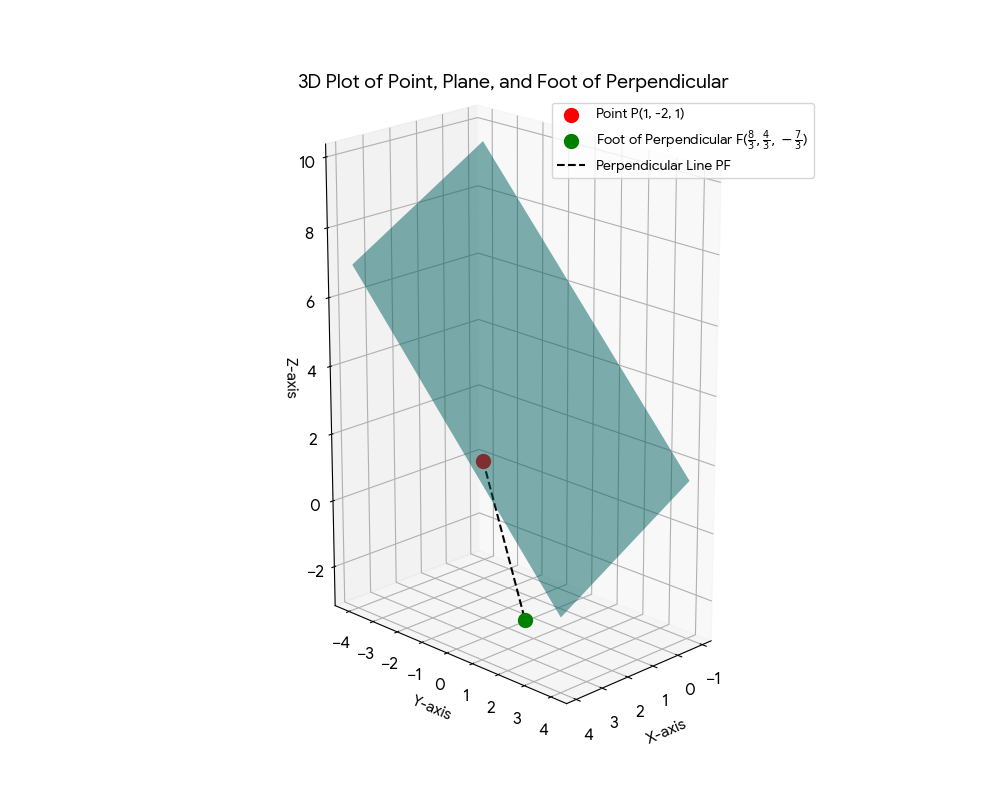
\includegraphics[width=\columnwidth, height=0.8\textheight, keepaspectratio]{figs/python_plot.png}     
\end{frame}


\end{document}